\documentclass[aspectratio=169]{beamer}

\usepackage{amsthm}
\usepackage{amssymb}
\usepackage{amsfonts}
\usepackage{amsmath}
\usepackage{mathtools}

\usepackage{pgf}
\usepgflibrary{fpu}
\usepackage{pgfplots}
\usepackage{tikz}
\usetikzlibrary{angles,fit,arrows,calc,math,matrix,intersections,through,backgrounds,cd}
\usepackage{tkz-euclide}
\usepackage{tkz-graph}
\usepackage{graphicx}
\pgfplotsset{compat=1.18}

\usetheme{Pittsburgh}
\usecolortheme{seahorse}

\title{Arithmetic expression geometry}
\author[Author] {Mingli Yuan}


\begin{document}
\pgfplotsset{compat=1.18}

\begin{frame}
\frametitle{Ancient Egyptian multiplication}
    The ancient Egyptian multiplication is a method involving only addition, doubling, and halving, which mixed 2-based and 10-based characteristics.
    \begin{figure}[ht]\centering
    \resizebox{0.6\textwidth}{!}{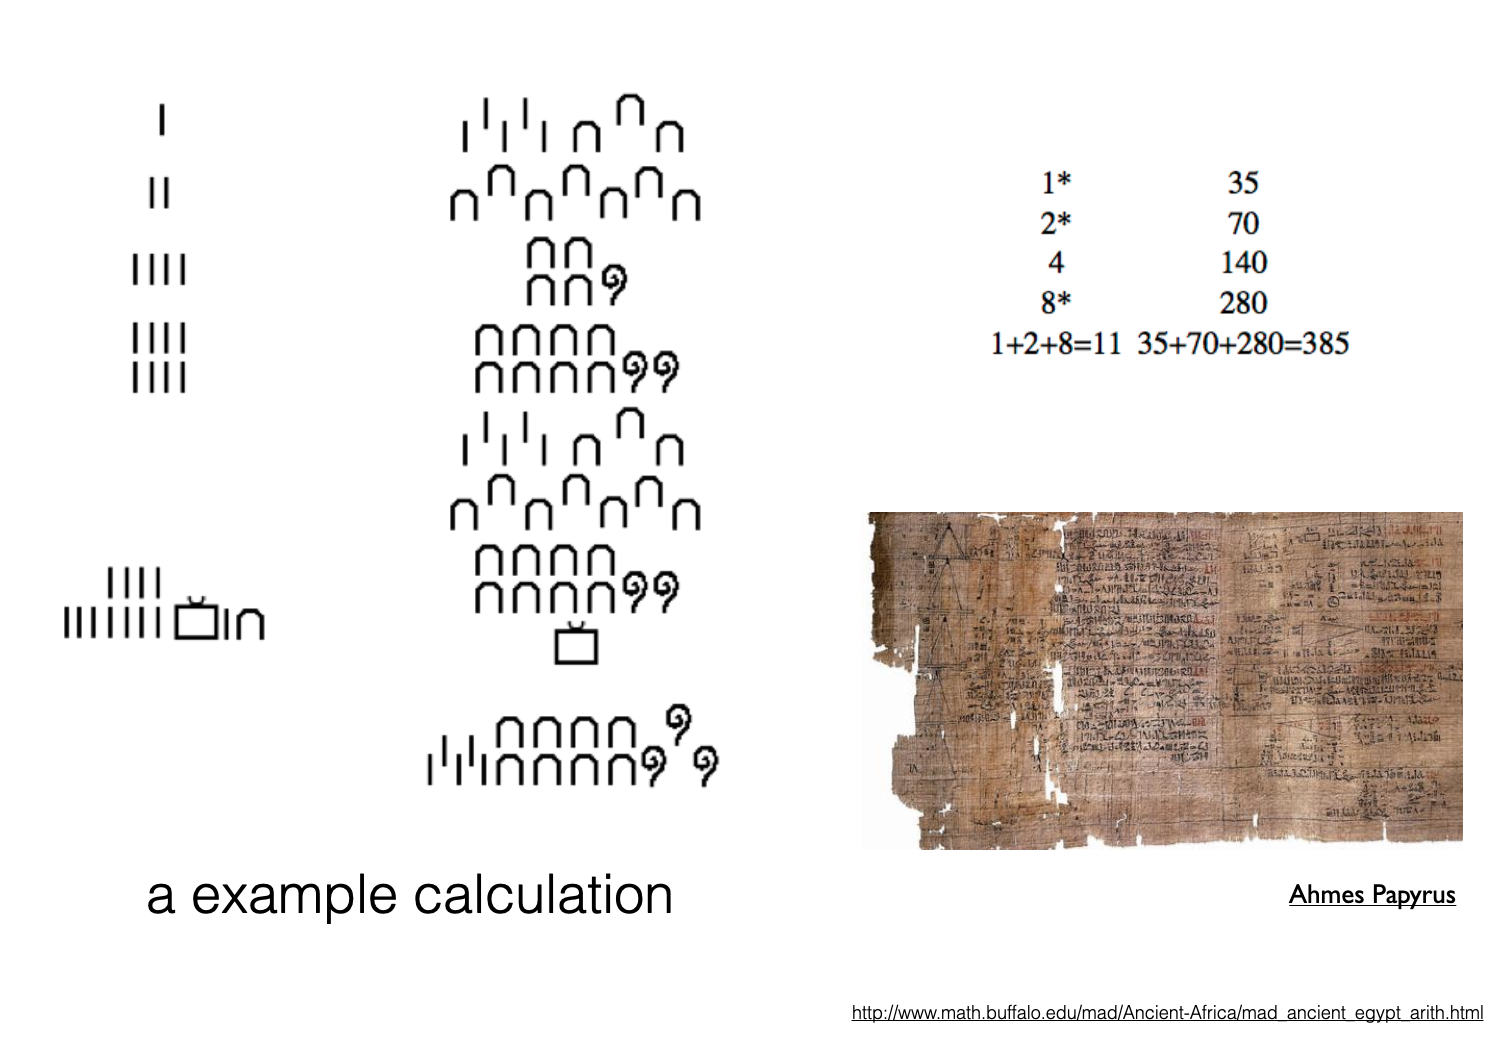
\includegraphics{images/egyptian.png}}
    \end{figure}
\end{frame}

\begin{frame}
\frametitle{A story of square root of 17}
A story from Plato's Theaetetus: Theodorus of Cyrene, a young mathematician, was able to prove that $\sqrt{3}$, $\sqrt{5}$... are irrational, but not $\sqrt{17}$.
\begin{columns}
\begin{column}{0.5\textwidth}
    \begin{figure}[ht]\centering
    \resizebox{0.6\textwidth}{!}{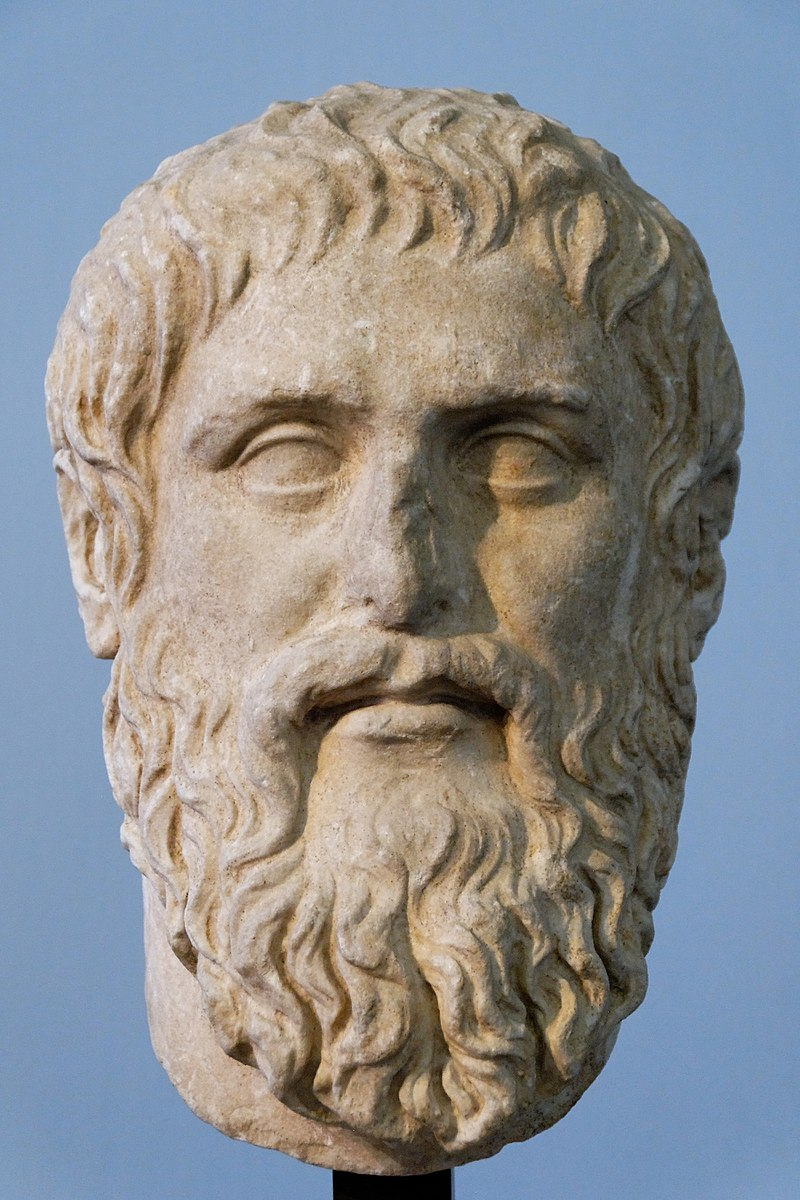
\includegraphics{images/Plato.jpeg}}
    \end{figure}
\end{column}
\begin{column}{0.5\textwidth}
    \begin{figure}[ht]\centering
    \resizebox{0.8\textwidth}{!}{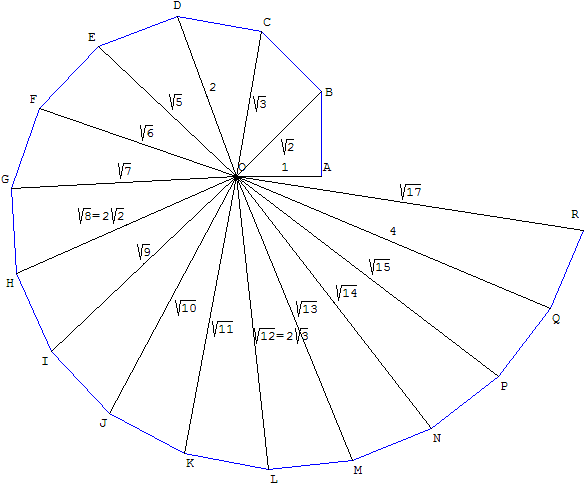
\includegraphics{images/escargot_pythagore.png}}
    \end{figure}
\end{column}
\end{columns}
\end{frame}

\begin{frame}
\frametitle{Prof. Pambuccian's axioms}
This story remained a mystery for more than 2000 years until Prof. Pambuccian's work published in 2012.
Prof. Pambuccian and Celia Schacht gave formal systems showed that irrationality of $\sqrt{17}$ is unprovable.
\begin{columns}
\begin{column}{0.4\textwidth}
    \begin{figure}[ht]\centering
    \resizebox{0.8\textwidth}{!}{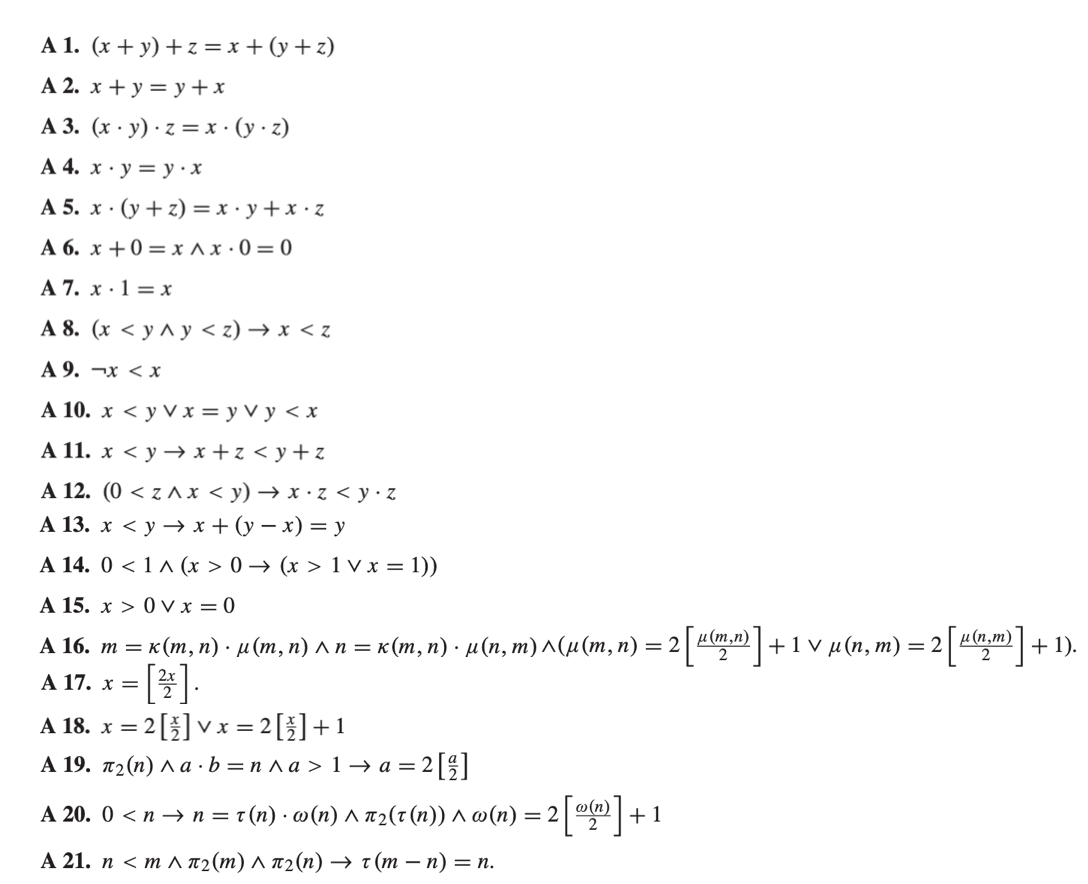
\includegraphics{images/axioms.png}}
    \end{figure}
\end{column}
\begin{column}{0.4\textwidth}
    \begin{itemize}
        \item A.1 - A.7 are involving arithmetic operations with equality.
        \item A.8 - A.15 are involving order relations.
        \item A.16 - A.22 are involving arithmetic functions related with odd and even.
    \end{itemize}
\end{column}
\end{columns}
\end{frame}

\begin{frame}
\frametitle{Embedding}
The axioms A.1 - A.7 are also fit into expressions, and then some terms of the formal system can be embedded into the expression space.
\begin{columns}
\begin{column}{0.7\textwidth}
\begin{figure}[ht]
\centering

\tikzmath{
  \one = 1;
  \base = 2;
  \offset = 15.8888888;
  \valofpi = 3.1415926;
  \anglei = 3.1415926;
  \angleo = 3.1415926;
}

\resizebox{0.8\columnwidth}{!}{%
\begin{tikzpicture}
\draw [black, line width=0.6pt, ->] (15.875,0) to[out=90,in=270] (15.875,6.3);
\node [anchor=south] at (15.875,6.3) {y};
\draw [black, line width=0.6pt, ->] (7,0) to[out=0,in=180] (18,0);
\node [anchor=west] at (18.3,0) {x};

\foreach \x in {-10,...,2}
  \node [anchor=north] at (\x / 9 * 8 + \offset,0) {\x};
\foreach \y in {1,...,6}
  \node [anchor=-135] at (6,\y / 9 * 8) {\y};

\foreach \t in {6, ..., 1}
  \draw [lightgray, line width=0.6pt] (7, \t / 9 * 8) to[out=0,in=180] (18, \t / 9 * 8);

\foreach \t in {-10, ..., 2}
  \draw [lightgray, line width=0.6pt] (\t / 9 * 8 + \offset, 0) to[out=90,in=270] (\t / 9 * 8 + \offset, 6);

\draw [green, line width=1.0pt] (-10 / 9 * 8 + \offset, 0) to[out=90,in=270] (-10 / 9 * 8 + \offset, 2 / 9 * 8);
\draw [green, line width=1.0pt] (-9 / 9 * 8 + \offset, 0) to[out=90,in=270] (-9 / 9 * 8 + \offset, 1 / 9 * 8);
\draw [green, line width=1.0pt] (-8 / 9 * 8 + \offset, 0) to[out=90,in=270] (-8 / 9 * 8 + \offset, 7 / 9 * 8);
\draw [green, line width=1.0pt] (-7 / 9 * 8 + \offset, 0) to[out=90,in=270] (-7 / 9 * 8 + \offset, 1 / 9 * 8);
\draw [green, line width=1.0pt] (-6 / 9 * 8 + \offset, 0) to[out=90,in=270] (-6 / 9 * 8 + \offset, 2 / 9 * 8);
\draw [green, line width=1.0pt] (-5 / 9 * 8 + \offset, 0) to[out=90,in=270] (-5 / 9 * 8 + \offset, 1 / 9 * 8);
\draw [green, line width=1.0pt] (-4 / 9 * 8 + \offset, 0) to[out=90,in=270] (-4 / 9 * 8 + \offset, 4 / 9 * 8);
\draw [green, line width=1.0pt] (-3 / 9 * 8 + \offset, 0) to[out=90,in=270] (-3 / 9 * 8 + \offset, 1 / 9 * 8);
\draw [green, line width=1.0pt] (-2 / 9 * 8 + \offset, 0) to[out=90,in=270] (-2 / 9 * 8 + \offset, 2 / 9 * 8);
\draw [green, line width=1.0pt] (-1 / 9 * 8 + \offset, 0) to[out=90,in=270] (-1 / 9 * 8 + \offset, 1 / 9 * 8);

\foreach \a in {4, 2, 1}
    \draw [blue, line width=0.6pt] (7, \a / 9 * 8) to[out=0,in=180] (18, \a / 9 * 8);

\node[circle,fill=black,inner sep=1pt,minimum size=3pt] (b) at (-4 / 9 * 8 + \offset, 4 / 9 * 8) {};
\node [anchor=315, red] at (-4 / 9 * 8 + \offset, 4 / 9 * 8) {1};
\node[circle,fill=black,inner sep=1pt,minimum size=3pt] (b) at (-8 / 9 * 8 + \offset, 4 / 9 * 8) {};
\node [anchor=315, red] at (-8 / 9 * 8 + \offset, 4 / 9 * 8) {2};

\node[circle,fill=black,inner sep=1pt,minimum size=3pt] (b) at (-2 / 9 * 8 + \offset, 2 / 9 * 8) {};
\node [anchor=315, red] at (-2 / 9 * 8 + \offset, 2 / 9 * 8) {1};
\node[circle,fill=black,inner sep=1pt,minimum size=3pt] (b) at (-4 / 9 * 8 + \offset, 2 / 9 * 8) {};
\node [anchor=315, red] at (-4 / 9 * 8 + \offset, 2 / 9 * 8) {2};
\node[circle,fill=black,inner sep=1pt,minimum size=3pt] (b) at (-6 / 9 * 8 + \offset, 2 / 9 * 8) {};
\node [anchor=315, red] at (-6 / 9 * 8 + \offset, 2 / 9 * 8) {3};

\node[circle,fill=black,inner sep=1pt,minimum size=3pt] (b) at (-1 / 9 * 8 + \offset, 1 / 9 * 8) {};
\node [anchor=315, red] at (-1 / 9 * 8 + \offset, 1 / 9 * 8) {1};
\node[circle,fill=black,inner sep=1pt,minimum size=3pt] (b) at (-2 / 9 * 8 + \offset, 1 / 9 * 8) {};
\node [anchor=315, red] at (-2 / 9 * 8 + \offset, 1 / 9 * 8) {2};
\node[circle,fill=black,inner sep=1pt,minimum size=3pt] (b) at (-3 / 9 * 8 + \offset, 1 / 9 * 8) {};
\node [anchor=315, red] at (-3 / 9 * 8 + \offset, 1 / 9 * 8) {3};
\node[circle,fill=black,inner sep=1pt,minimum size=3pt] (b) at (-4 / 9 * 8 + \offset, 1 / 9 * 8) {};
\node [anchor=315, red] at (-4 / 9 * 8 + \offset, 1 / 9 * 8) {4};
\node[circle,fill=black,inner sep=1pt,minimum size=3pt] (b) at (-5 / 9 * 8 + \offset, 1 / 9 * 8) {};
\node [anchor=315, red] at (-5 / 9 * 8 + \offset, 1 / 9 * 8) {5};
\node[circle,fill=black,inner sep=1pt,minimum size=3pt] (b) at (-6 / 9 * 8 + \offset, 1 / 9 * 8) {};
\node [anchor=315, red] at (-6 / 9 * 8 + \offset, 1 / 9 * 8) {6};

\draw [brown, line width=1.0pt] (1 / 9 * 8 + \offset, 3 / 9 * 8) to[out=251.5651,in=71.5651] (0 / 9 * 8 + \offset, 0 / 9 * 8);
\draw [brown, line width=1.0pt] (-9 / 9 * 8 + \offset, 3 / 9 * 8) to[out=-18.4349,in=161.5651] (0 / 9 * 8 + \offset, 0 / 9 * 8);
\node [anchor=315, red] at (1 / 9 * 8 + \offset, 3 / 9 * 8) {$\frac{1}{3}$};
\node [anchor=315, red] at (-9 / 9 * 8 + \offset, 3 / 9 * 8) {3};

\begin{scope}
    \clip (-10 / 9 * 8 + \offset,0) rectangle (2 / 9 * 8 + \offset, 6 / 9 * 8);
    \draw[purple,scale=1.0,samples=360,domain=0.0:360,variable=\t] plot ({- 0 / 2 / 9 * 8 + \offset + 2 / 2 / 9 * 8 * cos(\t) },{2 / 2 / 9 * 8 * sin(\t)});
    \draw[purple,scale=1.0,samples=360,domain=0.0:360,variable=\t] plot ({- 3 / 2 / 9 * 8 + \offset + 5 / 2 / 9 * 8 * cos(\t) },{5 / 2 / 9 * 8 * sin(\t)});
    \draw[purple,scale=1.0,samples=360,domain=0.0:360,variable=\t] plot ({- 8 / 2 / 9 * 8 + \offset + 10 / 2 / 9 * 8 * cos(\t) },{10 / 2 / 9 * 8 * sin(\t)});
\end{scope}

\end{tikzpicture}
}
\end{figure}
\end{column}
\end{columns}

\end{frame}

\begin{frame}
\frametitle{From proof theory to group theory?}
Can we migrate the problem of irrationality of $\sqrt{17}$ from proof theory into a problem in group theory?
\begin{columns}
\begin{column}{0.7\textwidth}
\begin{figure}[ht]
\centering

\tikzmath{
  \one = 1;
  \base = 2;
  \offset = 15.8888888;
  \valofpi = 3.1415926;
  \anglei = 3.1415926;
  \angleo = 3.1415926;
}

\resizebox{0.8\columnwidth}{!}{%
\begin{tikzpicture}
\draw [black, line width=0.6pt, ->] (15.875,0) to[out=90,in=270] (15.875,21.3);
\node [anchor=south] at (16,21.3) {y};
\draw [black, line width=0.6pt, ->] (-16.5,0) to[out=0,in=180] (18,0);
\node [anchor=west] at (18.5,0) {x};

\foreach \x in {-35,...,2}
  \node [anchor=north] at (\x / 9 * 8 + \offset,0) {\x};
\foreach \y in {1,...,21}
  \node [anchor=-135] at (18,\y / 9 * 8) {\y};

\foreach \t in {21, ..., 1}
  \draw [lightgray, line width=0.6pt] (-16.5, \t / 9 * 8) to[out=0,in=180] (18, \t / 9 * 8);

\foreach \t in {-36, ..., 2}
  \draw [lightgray, line width=0.6pt] (\t / 9 * 8 + \offset, 0) to[out=90,in=270] (\t / 9 * 8 + \offset, 21);

\draw [green, line width=1.0pt] (-36 / 9 * 8 + \offset, 0) to[out=90,in=270] (-36 / 9 * 8 + \offset, 4 / 9 * 8);
\draw [green, line width=1.0pt] (-35 / 9 * 8 + \offset, 0) to[out=90,in=270] (-35 / 9 * 8 + \offset, 1 / 9 * 8);
\draw [green, line width=1.0pt] (-34 / 9 * 8 + \offset, 0) to[out=90,in=270] (-34 / 9 * 8 + \offset, 2 / 9 * 8);
\draw [green, line width=1.0pt] (-33 / 9 * 8 + \offset, 0) to[out=90,in=270] (-33 / 9 * 8 + \offset, 1 / 9 * 8);
\draw [green, line width=1.0pt] (-31 / 9 * 8 + \offset, 0) to[out=90,in=270] (-31 / 9 * 8 + \offset, 1 / 9 * 8);
\draw [green, line width=1.0pt] (-30 / 9 * 8 + \offset, 0) to[out=90,in=270] (-30 / 9 * 8 + \offset, 2 / 9 * 8);
\draw [green, line width=1.0pt] (-29 / 9 * 8 + \offset, 0) to[out=90,in=270] (-29 / 9 * 8 + \offset, 1 / 9 * 8);
\draw [green, line width=1.0pt] (-28 / 9 * 8 + \offset, 0) to[out=90,in=270] (-28 / 9 * 8 + \offset, 4 / 9 * 8);
\draw [green, line width=1.0pt] (-27 / 9 * 8 + \offset, 0) to[out=90,in=270] (-27 / 9 * 8 + \offset, 1 / 9 * 8);
\draw [green, line width=1.0pt] (-26 / 9 * 8 + \offset, 0) to[out=90,in=270] (-26 / 9 * 8 + \offset, 2 / 9 * 8);
\draw [green, line width=1.0pt] (-25 / 9 * 8 + \offset, 0) to[out=90,in=270] (-25 / 9 * 8 + \offset, 1 / 9 * 8);
\draw [green, line width=1.0pt] (-24 / 9 * 8 + \offset, 0) to[out=90,in=270] (-24 / 9 * 8 + \offset, 8 / 9 * 8);
\draw [green, line width=1.0pt] (-23 / 9 * 8 + \offset, 0) to[out=90,in=270] (-23 / 9 * 8 + \offset, 1 / 9 * 8);
\draw [green, line width=1.0pt] (-22 / 9 * 8 + \offset, 0) to[out=90,in=270] (-22 / 9 * 8 + \offset, 2 / 9 * 8);
\draw [green, line width=1.0pt] (-21 / 9 * 8 + \offset, 0) to[out=90,in=270] (-21 / 9 * 8 + \offset, 1 / 9 * 8);
\draw [green, line width=1.0pt] (-20 / 9 * 8 + \offset, 0) to[out=90,in=270] (-20 / 9 * 8 + \offset, 4 / 9 * 8);
\draw [green, line width=1.0pt] (-19 / 9 * 8 + \offset, 0) to[out=90,in=270] (-19 / 9 * 8 + \offset, 1 / 9 * 8);
\draw [green, line width=1.0pt] (-18 / 9 * 8 + \offset, 0) to[out=90,in=270] (-18 / 9 * 8 + \offset, 2 / 9 * 8);
\draw [green, line width=1.0pt] (-17 / 9 * 8 + \offset, 0) to[out=90,in=270] (-17 / 9 * 8 + \offset, 1 / 9 * 8);
\draw [green, line width=1.0pt] (-16 / 9 * 8 + \offset, 0) to[out=90,in=270] (-16 / 9 * 8 + \offset, 16 / 9 * 8);
\draw [green, line width=1.0pt] (-15 / 9 * 8 + \offset, 0) to[out=90,in=270] (-15 / 9 * 8 + \offset, 1 / 9 * 8);
\draw [green, line width=1.0pt] (-14 / 9 * 8 + \offset, 0) to[out=90,in=270] (-14 / 9 * 8 + \offset, 2 / 9 * 8);
\draw [green, line width=1.0pt] (-13 / 9 * 8 + \offset, 0) to[out=90,in=270] (-13 / 9 * 8 + \offset, 1 / 9 * 8);
\draw [green, line width=1.0pt] (-12 / 9 * 8 + \offset, 0) to[out=90,in=270] (-12 / 9 * 8 + \offset, 4 / 9 * 8);
\draw [green, line width=1.0pt] (-11 / 9 * 8 + \offset, 0) to[out=90,in=270] (-11 / 9 * 8 + \offset, 1 / 9 * 8);
\draw [green, line width=1.0pt] (-10 / 9 * 8 + \offset, 0) to[out=90,in=270] (-10 / 9 * 8 + \offset, 2 / 9 * 8);
\draw [green, line width=1.0pt] (-9 / 9 * 8 + \offset, 0) to[out=90,in=270] (-9 / 9 * 8 + \offset, 1 / 9 * 8);
\draw [green, line width=1.0pt] (-8 / 9 * 8 + \offset, 0) to[out=90,in=270] (-8 / 9 * 8 + \offset, 8 / 9 * 8);
\draw [green, line width=1.0pt] (-7 / 9 * 8 + \offset, 0) to[out=90,in=270] (-7 / 9 * 8 + \offset, 1 / 9 * 8);
\draw [green, line width=1.0pt] (-6 / 9 * 8 + \offset, 0) to[out=90,in=270] (-6 / 9 * 8 + \offset, 2 / 9 * 8);
\draw [green, line width=1.0pt] (-5 / 9 * 8 + \offset, 0) to[out=90,in=270] (-5 / 9 * 8 + \offset, 1 / 9 * 8);
\draw [green, line width=1.0pt] (-4 / 9 * 8 + \offset, 0) to[out=90,in=270] (-4 / 9 * 8 + \offset, 4 / 9 * 8);
\draw [green, line width=1.0pt] (-3 / 9 * 8 + \offset, 0) to[out=90,in=270] (-3 / 9 * 8 + \offset, 1 / 9 * 8);
\draw [green, line width=1.0pt] (-2 / 9 * 8 + \offset, 0) to[out=90,in=270] (-2 / 9 * 8 + \offset, 2 / 9 * 8);
\draw [green, line width=1.0pt] (-1 / 9 * 8 + \offset, 0) to[out=90,in=270] (-1 / 9 * 8 + \offset, 1 / 9 * 8);

\foreach \a in {16, 8, 4, 2, 1}
    \draw [blue, line width=0.6pt] (-16.5, \a / 9 * 8) to[out=0,in=180] (18, \a / 9 * 8);

\node[circle,fill=black,inner sep=1pt,minimum size=3pt] (a) at (-16 / 9 * 8 + \offset, 16 / 9 * 8) {};
\node [anchor=315, red] at (-16 / 9 * 8 + \offset, 16 / 9 * 8) {1};
\node[circle,fill=black,inner sep=1pt,minimum size=3pt] (a) at (-16 / 9 * 8 + \offset, 16 / 9 * 8) {};
\node [anchor=315, red] at (-32 / 9 * 8 + \offset, 16 / 9 * 8) {2};

\node[circle,fill=black,inner sep=1pt,minimum size=3pt] (b) at (-8 / 9 * 8 + \offset, 8 / 9 * 8) {};
\node [anchor=315, red] at (-8 / 9 * 8 + \offset, 8 / 9 * 8) {1};
\node[circle,fill=black,inner sep=1pt,minimum size=3pt] (b) at (-16 / 9 * 8 + \offset, 8 / 9 * 8) {};
\node [anchor=315, red] at (-16 / 9 * 8 + \offset, 8 / 9 * 8) {2};
\node[circle,fill=black,inner sep=1pt,minimum size=3pt] (b) at (-16 / 9 * 8 + \offset, 8 / 9 * 8) {};
\node [anchor=315, red] at (-24 / 9 * 8 + \offset, 8 / 9 * 8) {3};
\node[circle,fill=black,inner sep=1pt,minimum size=3pt] (b) at (-16 / 9 * 8 + \offset, 8 / 9 * 8) {};
\node [anchor=315, red] at (-32 / 9 * 8 + \offset, 8 / 9 * 8) {4};

\node[circle,fill=black,inner sep=1pt,minimum size=3pt] (b) at (-4 / 9 * 8 + \offset, 4 / 9 * 8) {};
\node [anchor=315, red] at (-4 / 9 * 8 + \offset, 4 / 9 * 8) {1};
\node[circle,fill=black,inner sep=1pt,minimum size=3pt] (b) at (-8 / 9 * 8 + \offset, 4 / 9 * 8) {};
\node [anchor=315, red] at (-8 / 9 * 8 + \offset, 4 / 9 * 8) {2};
\node[circle,fill=black,inner sep=1pt,minimum size=3pt] (b) at (-12 / 9 * 8 + \offset, 4 / 9 * 8) {};
\node [anchor=315, red] at (-12 / 9 * 8 + \offset, 4 / 9 * 8) {3};
\node[circle,fill=black,inner sep=1pt,minimum size=3pt] (b) at (-16 / 9 * 8 + \offset, 4 / 9 * 8) {};
\node [anchor=315, red] at (-16 / 9 * 8 + \offset, 4 / 9 * 8) {4};
\node[circle,fill=black,inner sep=1pt,minimum size=3pt] (b) at (-20 / 9 * 8 + \offset, 4 / 9 * 8) {};
\node [anchor=315, red] at (-20 / 9 * 8 + \offset, 4 / 9 * 8) {5};
\node[circle,fill=black,inner sep=1pt,minimum size=3pt] (b) at (-24 / 9 * 8 + \offset, 4 / 9 * 8) {};
\node [anchor=315, red] at (-24 / 9 * 8 + \offset, 4 / 9 * 8) {6};
\node[circle,fill=black,inner sep=1pt,minimum size=3pt] (b) at (-28 / 9 * 8 + \offset, 4 / 9 * 8) {};
\node [anchor=315, red] at (-28 / 9 * 8 + \offset, 4 / 9 * 8) {7};
\node[circle,fill=black,inner sep=1pt,minimum size=3pt] (b) at (-32 / 9 * 8 + \offset, 4 / 9 * 8) {};
\node [anchor=315, red] at (-32 / 9 * 8 + \offset, 4 / 9 * 8) {8};
\node[circle,fill=black,inner sep=1pt,minimum size=3pt] (b) at (-36 / 9 * 8 + \offset, 4 / 9 * 8) {};
\node [anchor=315, red] at (-36 / 9 * 8 + \offset, 4 / 9 * 8) {9};

\node[circle,fill=black,inner sep=1pt,minimum size=3pt] (b) at (-2 / 9 * 8 + \offset, 2 / 9 * 8) {};
\node [anchor=315, red] at (-2 / 9 * 8 + \offset, 2 / 9 * 8) {1};
\node[circle,fill=black,inner sep=1pt,minimum size=3pt] (b) at (-4 / 9 * 8 + \offset, 2 / 9 * 8) {};
\node [anchor=315, red] at (-4 / 9 * 8 + \offset, 2 / 9 * 8) {2};
\node[circle,fill=black,inner sep=1pt,minimum size=3pt] (b) at (-6 / 9 * 8 + \offset, 2 / 9 * 8) {};
\node [anchor=315, red] at (-6 / 9 * 8 + \offset, 2 / 9 * 8) {3};
\node[circle,fill=black,inner sep=1pt,minimum size=3pt] (b) at (-8 / 9 * 8 + \offset, 2 / 9 * 8) {};
\node [anchor=315, red] at (-8 / 9 * 8 + \offset, 2 / 9 * 8) {4};
\node[circle,fill=black,inner sep=1pt,minimum size=3pt] (b) at (-10 / 9 * 8 + \offset, 2 / 9 * 8) {};
\node [anchor=315, red] at (-10 / 9 * 8 + \offset, 2 / 9 * 8) {5};
\node[circle,fill=black,inner sep=1pt,minimum size=3pt] (b) at (-12 / 9 * 8 + \offset, 2 / 9 * 8) {};
\node [anchor=315, red] at (-12 / 9 * 8 + \offset, 2 / 9 * 8) {6};
\node[circle,fill=black,inner sep=1pt,minimum size=3pt] (b) at (-14 / 9 * 8 + \offset, 2 / 9 * 8) {};
\node [anchor=315, red] at (-14 / 9 * 8 + \offset, 2 / 9 * 8) {7};
\node[circle,fill=black,inner sep=1pt,minimum size=3pt] (b) at (-16 / 9 * 8 + \offset, 2 / 9 * 8) {};
\node [anchor=315, red] at (-16 / 9 * 8 + \offset, 2 / 9 * 8) {8};
\node[circle,fill=black,inner sep=1pt,minimum size=3pt] (b) at (-18 / 9 * 8 + \offset, 2 / 9 * 8) {};
\node [anchor=315, red] at (-18 / 9 * 8 + \offset, 2 / 9 * 8) {9};
\node[circle,fill=black,inner sep=1pt,minimum size=3pt] (b) at (-20 / 9 * 8 + \offset, 2 / 9 * 8) {};
\node [anchor=315, red] at (-20 / 9 * 8 + \offset, 2 / 9 * 8) {10};
\node[circle,fill=black,inner sep=1pt,minimum size=3pt] (b) at (-22 / 9 * 8 + \offset, 2 / 9 * 8) {};
\node [anchor=315, red] at (-22 / 9 * 8 + \offset, 2 / 9 * 8) {11};
\node[circle,fill=black,inner sep=1pt,minimum size=3pt] (b) at (-24 / 9 * 8 + \offset, 2 / 9 * 8) {};
\node [anchor=315, red] at (-24 / 9 * 8 + \offset, 2 / 9 * 8) {12};
\node[circle,fill=black,inner sep=1pt,minimum size=3pt] (b) at (-26 / 9 * 8 + \offset, 2 / 9 * 8) {};
\node [anchor=315, red] at (-26 / 9 * 8 + \offset, 2 / 9 * 8) {13};
\node[circle,fill=black,inner sep=1pt,minimum size=3pt] (b) at (-28 / 9 * 8 + \offset, 2 / 9 * 8) {};
\node [anchor=315, red] at (-28 / 9 * 8 + \offset, 2 / 9 * 8) {14};
\node[circle,fill=black,inner sep=1pt,minimum size=3pt] (b) at (-30 / 9 * 8 + \offset, 2 / 9 * 8) {};
\node [anchor=315, red] at (-30 / 9 * 8 + \offset, 2 / 9 * 8) {15};
\node[circle,fill=black,inner sep=1pt,minimum size=3pt] (b) at (-32 / 9 * 8 + \offset, 2 / 9 * 8) {};
\node [anchor=315, red] at (-32 / 9 * 8 + \offset, 2 / 9 * 8) {16};
\node[circle,fill=black,inner sep=1pt,minimum size=3pt] (b) at (-34 / 9 * 8 + \offset, 2 / 9 * 8) {};
\node [anchor=315, red] at (-34 / 9 * 8 + \offset, 2 / 9 * 8) {17};
\node[circle,fill=black,inner sep=1pt,minimum size=3pt] (b) at (-36 / 9 * 8 + \offset, 2 / 9 * 8) {};
\node [anchor=315, red] at (-36 / 9 * 8 + \offset, 2 / 9 * 8) {18};

\node[circle,fill=black,inner sep=1pt,minimum size=3pt] (b) at (-1 / 9 * 8 + \offset, 1 / 9 * 8) {};
\node [anchor=315, red] at (-1 / 9 * 8 + \offset, 1 / 9 * 8) {1};
\node[circle,fill=black,inner sep=1pt,minimum size=3pt] (b) at (-2 / 9 * 8 + \offset, 1 / 9 * 8) {};
\node [anchor=315, red] at (-2 / 9 * 8 + \offset, 1 / 9 * 8) {2};
\node[circle,fill=black,inner sep=1pt,minimum size=3pt] (b) at (-3 / 9 * 8 + \offset, 1 / 9 * 8) {};
\node [anchor=315, red] at (-3 / 9 * 8 + \offset, 1 / 9 * 8) {3};
\node[circle,fill=black,inner sep=1pt,minimum size=3pt] (b) at (-4 / 9 * 8 + \offset, 1 / 9 * 8) {};
\node [anchor=315, red] at (-4 / 9 * 8 + \offset, 1 / 9 * 8) {4};
\node[circle,fill=black,inner sep=1pt,minimum size=3pt] (b) at (-5 / 9 * 8 + \offset, 1 / 9 * 8) {};
\node [anchor=315, red] at (-5 / 9 * 8 + \offset, 1 / 9 * 8) {5};
\node[circle,fill=black,inner sep=1pt,minimum size=3pt] (b) at (-6 / 9 * 8 + \offset, 1 / 9 * 8) {};
\node [anchor=315, red] at (-6 / 9 * 8 + \offset, 1 / 9 * 8) {6};
\node[circle,fill=black,inner sep=1pt,minimum size=3pt] (b) at (-7 / 9 * 8 + \offset, 1 / 9 * 8) {};
\node [anchor=315, red] at (-7 / 9 * 8 + \offset, 1 / 9 * 8) {7};
\node[circle,fill=black,inner sep=1pt,minimum size=3pt] (b) at (-8 / 9 * 8 + \offset, 1 / 9 * 8) {};
\node [anchor=315, red] at (-8 / 9 * 8 + \offset, 1 / 9 * 8) {8};
\node[circle,fill=black,inner sep=1pt,minimum size=3pt] (b) at (-9 / 9 * 8 + \offset, 1 / 9 * 8) {};
\node [anchor=315, red] at (-9 / 9 * 8 + \offset, 1 / 9 * 8) {9};
\node[circle,fill=black,inner sep=1pt,minimum size=3pt] (b) at (-10 / 9 * 8 + \offset, 1 / 9 * 8) {};
\node [anchor=315, red] at (-10 / 9 * 8 + \offset, 1 / 9 * 8) {10};
\node[circle,fill=black,inner sep=1pt,minimum size=3pt] (b) at (-11 / 9 * 8 + \offset, 1 / 9 * 8) {};
\node [anchor=315, red] at (-11 / 9 * 8 + \offset, 1 / 9 * 8) {11};
\node[circle,fill=black,inner sep=1pt,minimum size=3pt] (b) at (-12 / 9 * 8 + \offset, 1 / 9 * 8) {};
\node [anchor=315, red] at (-12 / 9 * 8 + \offset, 1 / 9 * 8) {12};
\node[circle,fill=black,inner sep=1pt,minimum size=3pt] (b) at (-13 / 9 * 8 + \offset, 1 / 9 * 8) {};
\node [anchor=315, red] at (-13 / 9 * 8 + \offset, 1 / 9 * 8) {13};
\node[circle,fill=black,inner sep=1pt,minimum size=3pt] (b) at (-14 / 9 * 8 + \offset, 1 / 9 * 8) {};
\node [anchor=315, red] at (-14 / 9 * 8 + \offset, 1 / 9 * 8) {14};
\node[circle,fill=black,inner sep=1pt,minimum size=3pt] (b) at (-15 / 9 * 8 + \offset, 1 / 9 * 8) {};
\node [anchor=315, red] at (-15 / 9 * 8 + \offset, 1 / 9 * 8) {15};
\node[circle,fill=black,inner sep=1pt,minimum size=3pt] (b) at (-16 / 9 * 8 + \offset, 1 / 9 * 8) {};
\node [anchor=315, red] at (-16 / 9 * 8 + \offset, 1 / 9 * 8) {16};
\node[circle,fill=black,inner sep=1pt,minimum size=3pt] (b) at (-17 / 9 * 8 + \offset, 1 / 9 * 8) {};
\node [anchor=315, red] at (-17 / 9 * 8 + \offset, 1 / 9 * 8) {17};
\node[circle,fill=black,inner sep=1pt,minimum size=3pt] (b) at (-18 / 9 * 8 + \offset, 1 / 9 * 8) {};
\node [anchor=315, red] at (-18 / 9 * 8 + \offset, 1 / 9 * 8) {18};
\node[circle,fill=black,inner sep=1pt,minimum size=3pt] (b) at (-19 / 9 * 8 + \offset, 1 / 9 * 8) {};
\node [anchor=315, red] at (-19 / 9 * 8 + \offset, 1 / 9 * 8) {19};
\node[circle,fill=black,inner sep=1pt,minimum size=3pt] (b) at (-20 / 9 * 8 + \offset, 1 / 9 * 8) {};
\node [anchor=315, red] at (-20 / 9 * 8 + \offset, 1 / 9 * 8) {20};
\node[circle,fill=black,inner sep=1pt,minimum size=3pt] (b) at (-21 / 9 * 8 + \offset, 1 / 9 * 8) {};
\node [anchor=315, red] at (-21 / 9 * 8 + \offset, 1 / 9 * 8) {21};
\node[circle,fill=black,inner sep=1pt,minimum size=3pt] (b) at (-22 / 9 * 8 + \offset, 1 / 9 * 8) {};
\node [anchor=315, red] at (-22 / 9 * 8 + \offset, 1 / 9 * 8) {22};
\node[circle,fill=black,inner sep=1pt,minimum size=3pt] (b) at (-23 / 9 * 8 + \offset, 1 / 9 * 8) {};
\node [anchor=315, red] at (-23 / 9 * 8 + \offset, 1 / 9 * 8) {23};
\node[circle,fill=black,inner sep=1pt,minimum size=3pt] (b) at (-24 / 9 * 8 + \offset, 1 / 9 * 8) {};
\node [anchor=315, red] at (-24 / 9 * 8 + \offset, 1 / 9 * 8) {24};
\node[circle,fill=black,inner sep=1pt,minimum size=3pt] (b) at (-25 / 9 * 8 + \offset, 1 / 9 * 8) {};
\node [anchor=315, red] at (-25 / 9 * 8 + \offset, 1 / 9 * 8) {25};
\node[circle,fill=black,inner sep=1pt,minimum size=3pt] (b) at (-26 / 9 * 8 + \offset, 1 / 9 * 8) {};
\node [anchor=315, red] at (-26 / 9 * 8 + \offset, 1 / 9 * 8) {26};
\node[circle,fill=black,inner sep=1pt,minimum size=3pt] (b) at (-27 / 9 * 8 + \offset, 1 / 9 * 8) {};
\node [anchor=315, red] at (-27 / 9 * 8 + \offset, 1 / 9 * 8) {27};
\node[circle,fill=black,inner sep=1pt,minimum size=3pt] (b) at (-28 / 9 * 8 + \offset, 1 / 9 * 8) {};
\node [anchor=315, red] at (-28 / 9 * 8 + \offset, 1 / 9 * 8) {28};
\node[circle,fill=black,inner sep=1pt,minimum size=3pt] (b) at (-29 / 9 * 8 + \offset, 1 / 9 * 8) {};
\node [anchor=315, red] at (-29 / 9 * 8 + \offset, 1 / 9 * 8) {29};
\node[circle,fill=black,inner sep=1pt,minimum size=3pt] (b) at (-30 / 9 * 8 + \offset, 1 / 9 * 8) {};
\node [anchor=315, red] at (-30 / 9 * 8 + \offset, 1 / 9 * 8) {30};
\node[circle,fill=black,inner sep=1pt,minimum size=3pt] (b) at (-31 / 9 * 8 + \offset, 1 / 9 * 8) {};
\node [anchor=315, red] at (-31 / 9 * 8 + \offset, 1 / 9 * 8) {31};
\node[circle,fill=black,inner sep=1pt,minimum size=3pt] (b) at (-32 / 9 * 8 + \offset, 1 / 9 * 8) {};
\node [anchor=315, red] at (-32 / 9 * 8 + \offset, 1 / 9 * 8) {32};
\node[circle,fill=black,inner sep=1pt,minimum size=3pt] (b) at (-33 / 9 * 8 + \offset, 1 / 9 * 8) {};
\node [anchor=315, red] at (-33 / 9 * 8 + \offset, 1 / 9 * 8) {33};
\node[circle,fill=black,inner sep=1pt,minimum size=3pt] (b) at (-34 / 9 * 8 + \offset, 1 / 9 * 8) {};
\node [anchor=315, red] at (-34 / 9 * 8 + \offset, 1 / 9 * 8) {34};
\node[circle,fill=black,inner sep=1pt,minimum size=3pt] (b) at (-35 / 9 * 8 + \offset, 1 / 9 * 8) {};
\node [anchor=315, red] at (-35 / 9 * 8 + \offset, 1 / 9 * 8) {35};
\node[circle,fill=black,inner sep=1pt,minimum size=3pt] (b) at (-36 / 9 * 8 + \offset, 1 / 9 * 8) {};
\node [anchor=315, red] at (-36 / 9 * 8 + \offset, 1 / 9 * 8) {36};

\draw [brown, line width=1.0pt] (1 / 9 * 8 + \offset, 3 / 9 * 8) to[out=251.5651,in=71.5651] (0 / 9 * 8 + \offset, 0 / 9 * 8);
\draw [brown, line width=1.0pt] (-9 / 9 * 8 + \offset, 3 / 9 * 8) to[out=-18.4349,in=161.5651] (0 / 9 * 8 + \offset, 0 / 9 * 8);

\begin{scope}
    \clip (-36 / 9 * 8 + \offset,0) rectangle (2 / 9 * 8 + \offset, 22 / 9 * 8);
    \draw[purple,scale=1.0,samples=360,domain=0.0:360,variable=\t] plot ({- 0 / 2 / 9 * 8 + \offset + 2 / 2 / 9 * 8 * cos(\t) },{2 / 2 / 9 * 8 * sin(\t)});
    \draw[purple,scale=1.0,samples=360,domain=0.0:360,variable=\t] plot ({- 3 / 2 / 9 * 8 + \offset + 5 / 2 / 9 * 8 * cos(\t) },{5 / 2 / 9 * 8 * sin(\t)});
    \draw[purple,scale=1.0,samples=360,domain=0.0:360,variable=\t] plot ({- 8 / 2 / 9 * 8 + \offset + 10 / 2 / 9 * 8 * cos(\t) },{10 / 2 / 9 * 8 * sin(\t)});
    \draw[purple,scale=1.0,samples=360,domain=0.0:360,variable=\t] plot ({- 15 / 2 / 9 * 8 + \offset + 17 / 2 / 9 * 8 * cos(\t) },{17 / 2 / 9 * 8 * sin(\t)});
    \draw[purple,scale=1.0,samples=360,domain=0.0:360,variable=\t] plot ({- 16 / 2 / 9 * 8 + \offset + 18 / 2 / 9 * 8 * cos(\t) },{18 / 2 / 9 * 8 * sin(\t)});
    \draw[purple,scale=1.0,samples=360,domain=0.0:360,variable=\t] plot ({- 24 / 2 / 9 * 8 + \offset + 26 / 2 / 9 * 8 * cos(\t) },{26 / 2 / 9 * 8 * sin(\t)});
    \draw[purple,scale=1.0,samples=360,domain=0.0:360,variable=\t] plot ({- 35 / 2 / 9 * 8 + \offset + 37 / 2 / 9 * 8 * cos(\t) },{37 / 2 / 9 * 8 * sin(\t)});
\end{scope}

\end{tikzpicture}
}
\end{figure}
\end{column}
\end{columns}

\end{frame}

\end{document}
